% Instructions for Authors fuer Acta Acustica


\documentclass[twoside,twocolumn]{article}
\usepackage{acta}
\usepackage{url}
\usepackage[utf8]{inputenc}
\usepackage{setspace}

\begin{document}
\Eingang{00}{00}{0000} \Annahme{00}{00}{0000} \Sachgebiet{1}
\PACS{43.50.Lj, 43.50.Rq, 43.50.Qp, 43.66.Lj, 43.66.Ba}
\Band{0} \Jahr{0000} \Heft{} \Ersteseite{1} \Letzteseite{}

\AuthorsI{G. Lafay$^{1)}$, M. Rossignol$^{2)}$, N. Misdariis$^{2)}$, M. Lagrange$^{1)}$, J.F. Petiot$^{1)}$}
\AddressI{$^{1)}$ Institut de Recherche en Communications et  Cybern\'etique de Nantes (IRCCYN), Nantes, France.\\
\hspace*{8pt}gregoire.lafay@irccyn.ec-nantes.fr\\
$^{2)}$ STMS Ircam-CNRS-UPMC Institut de Recherche et Coordination Acoustique/Musique, Paris, France}

% \footnotemark[1] \Authornotes{\footnotetext[1]{} }

\newcommand{\gl}[1]{\textcolor{blue}{GL : #1}}
\newcommand{\nm}[1]{\textcolor{red}{nm : #1}}
\newcommand{\ml}[1]{\textcolor{magenta}{ML : #1}}
\newcommand{\mr}[1]{\textcolor{green}{MR : #1}}

\Englishtitle{Investigating soundscapes perception through acoustic scenes simulation. Part I: simulation protocol presentation and case study} \Germanorfrenchtitle{}

\Kolumnentitel{Lafay et al. : Approaching mental representations}

\Englishabstract{This paper introduces a new experimental protocol to study mental representations of urban soundscapes through a simulation process. Subjects are asked to create a full soundscape by means of a  software dedicated to sound \gl{edition}, coupled with a structured sound data set. This paradigm is used to characterize urban sound environment representations by analyzing the sound classes that were used to simulate the auditory scenes. A rating experiment of the soundscape pleasantness using a 7-points bipolar scale is conducted to further refine the analysis of the simulated urban acoustic scenes. Results show that 1) a semantic characterization in terms of presence~/ absence of sound sources is an effective way to characterize urban soundscapes pleasantness, and 2) physical descriptors computed for specific sound sources better characterize the appraisal than global descriptors.}
\Germanorfrenchabstract{}

\ScientificPaper



%%%%%%%%%%%%%%%%%%%%%%%%%%%%%%%%%%%%%%%%%%%%%%%%%%%%%%%%%%%%
%%%%%%%%%%%%%%%%%%%%   INTRODUCTION      %%%%%%%%%%%%%%%%%%%
%%%%%%%%%%%%%%%%%%%%%%%%%%%%%%%%%%%%%%%%%%%%%%%%%%%%%%%%%%%%

%\onecolumn
\setlength{\parindent}{5ex}
%\setstretch{2}
\section{Introduction}

%% Original intro

%% The notion of soundscape has been introduced by Schafer \cite{schafer_new_1969, schafer1977tuning} in the 1970s as the auditory equivalent to landscape. Following this paradigm, a sonic environment is described by focusing on the listener's evaluation, rather than only taking into account the acoustic parameters of the sound. 

%% Only during the 1980s did policy-makers started taking into account the link between \textit{noise} and pollution, considering noise as a significant degradation of the quality of life. To fight this phenomenon, the first approach consisted in identifying unwanted sounds, and lowering their intensities. Thus, in the wake of this realization, several regulations have emerged, often limited to enforcing sound level thresholds. 

%% However, it is now widely accepted that acoustic comfort is a complex concept that cannot be described solely with the help of objective acoustical measures such as $LA_{(eq,V)}$, but needs to take into account other perceptive factors \cite{schulte-fortkamp_soundscape_2006, aletta2016soundscape, Yang2005211, kang_semantic_2010}. ``\,Noise\,''  is a cognitive object which depends upon a listener's appreciation and the context in which it is heard. Many urban ``\,noises\,'', such as that of a siren, can annoy as well as warn of a danger, and many town districts are appreciated because of a lively and animated atmosphere which often results in higher sound levels. Conventional noise regulations concentrate on high sound levels from transportation and industry, and their scope does not extend beyond unwanted sound sources. In other words, they do not try to improve the sonic environment by identifying and reinforcing pleasant or important sounds. This latter approach was pioneered by Schafer, who named it the ``\,positive\,'' approach. 

%% For two decades, the soundscape paradigm has been considered to study the perception of acoustic scenes in order to provide urban planners with meaningful sound quality indicators (see \cite{dubois2006cognitive} and  \cite{aletta2016soundscape} for extensive reviews). Most studies follow the \emph{modus operandi} of cognitive psychology \cite{maffiolo_caracterisation_1999}, by first describing the soundscape using both acoustic measurements and perceptive factors, and then investigating the interactions between those descriptors to understand the cognitive processes involved in the perception of the acoustic scenes. Soundscape studies are thus interdisciplinary \cite{davies_perception_2013, aletta2016soundscape}, borrowing tools from various fields such as acoustics, psycho-physics or cognitive psychology, but also psycho-linguistics, sociology and data mining. 

%% The soundscape approach appears to be a powerful tool to develop perceptively motivated indicators \cite{schulte-fortkamp_soundscape:_2007}. That said, the use of various experimental protocols to assess and measure soundscapes makes the integration of results difficult \cite{davies_perception_2013}. Also, there still exist no definite consensus in the soundscape community about the acoustic descriptors to be used \cite{aletta2016soundscape}. This issue prevents experimenters to provide  urban planners with generic and clear indicators or models able to predict sound environment quality \cite{schulte-fortkamp_soundscape:_2007, aletta2016soundscape}. Recently, several projects such as the European Cooperation in Science and Technology Action (TD0804: soundscape of European Cities and Landscapes) or the Positive Soundscape project \cite{davies_perception_2013} have been undertaken to standardize soundscape assessment and descriptors \cite{schulte2013soundscape}, but those matters are still considered as open problems.

%% We believe that soundscapes studies greatly suffer from one important issue: to the best of our knowledge, there is no morphological definition of a soundscape, and therefore no standardized way to decompose it in distinct elements. It is thus difficult to study precisely which component of the environment is the cause of potential variations in the perceptive measurements. 

%% We propose to tackle this issue by introducing a new experimental protocol, in which  subjects are asked to create a complex sonic environment thanks to a dedicated software tool linked to a dataset of isolated environmental sound samples. The simulation provides us with simulated scenes fully annotated in terms of source presence and sound levels. Those annotations enable us to ground the analyses of further perceptive descriptors obtained via standard perceptive evaluations of the simulated scenes, as well as to study the contribution of each sound source.

%% As a case study, we focus in this paper on urban soundscape pleasantness. We first give an overview of the tools used in soundscape perception studies, and justify the benefits of conducting this kind of simulation experiment as a data generation process. We then describe the simulation process, and present the results of the case study. The latter consists of two experiments: 1) a simulation experiment where subjects generate both ideal and non-ideal urban sonic environments, and 2) a pleasantness evaluation of the simulated scenes using a 7 points bipolar semantic scale.

%% Results show that 1) outcomes identified in the literature \cite{guastavino_categorization_2007} can be achieved by this approach, providing evidence that it has solid grounding,  2) sound markers that greatly affect the pleasantness of the soundscape can be identified with a good level of categorical detail, and 3) that physical descriptors computed specifically on the sound markers better characterise the appraisal than global descriptors.



%% Version MR 19/05/2016

The study of our sonic environments, both natural and man-made, has gathered growing interest in the past decades, finding applications in fields as varied as context inference and surveillance \cite{heittola13,1540194,park14}, evaluation of urban noise pollution \cite{raimbault_urban_2005} or the emerging area of eco-acoustics \cite{ECOACOUSTICS2014, krause}. The notion of \emph{soundscape}, introduced by Schafer \cite{schafer_new_1969, schafer1977tuning} in the 1970s as the auditory equivalent to landscape, is a theoretical framework of choice for that research. Following this paradigm, a sonic environment is described by focusing on the listener's evaluation \gl{and perception}, rather than only taking into account the acoustic parameters of the sound scene. 

Most soundscape studies follow the \emph{modus operandi} of cognitive psychology \cite{maffiolo_caracterisation_1999}, by first describing the soundscape using both acoustic measurements and perceptual factors, and then investigating the interactions between those descriptors to understand the cognitive processes involved in the perception of the acoustic scenes. Soundscape studies are thus interdisciplinary \cite{davies_perception_2013, aletta2016soundscape}, borrowing tools from various fields such as acoustics, psychophysics or cognitive psychology, but also psycho-linguistics, sociology and data mining. 

While the soundscape approach appears to be a powerful tool to develop perceptively motivated indicators \cite{schulte-fortkamp_soundscape:_2007}, the use of various experimental protocols to assess and measure soundscapes makes the integration of results difficult \cite{davies_perception_2013}. Moreover, there still exist no definite consensus in the soundscape community about the acoustic descriptors to be used \cite{brocolini2012prediction,aletta2016soundscape}. We believe that soundscapes studies greatly suffer from one important issue: to the best of our knowledge, there is no morphological definition of a soundscape, and therefore no standardized way to decompose it into distinct elements. It is thus difficult to study precisely which component of the environment is the cause of potential variations in the perceptual measurements.

We propose to tackle this issue by introducing a new experimental protocol, in which subjects are asked to create a complex sonic environment thanks to a dedicated software tool linked to a dataset of isolated environmental sound samples. The simulation provides us with simulated scenes fully annotated in terms of source presence and sound levels. Those annotations enable us to ground the analyses of further perceptual descriptors obtained via standard perceptual evaluations of the simulated scenes, as well as to study the contribution of each sound source.

As a case study to demonstrate the interest of that new approach, we focus in this paper on the issue of urban soundscape pleasantness as tackled in \cite{guastavino_ideal_2006} \nm{dans [14], il est plutot question de ideal / non ideal urban soundscapes ..... }.

Only during the 1980s did policy-makers start taking into account the link between \gl{``\,community noise\,''} and pollution, considering noise as a significant degradation of the life quality. To fight this phenomenon, the first approach consisted in identifying unwanted sounds, and lowering their intensities. Thus, in the wake of this realization, several regulations have emerged, often limited to enforcing sound level thresholds. 

However, it is now widely accepted that acoustic comfort is a complex concept that cannot be described solely with the help of objective acoustical measures such as $L_{Aeq}$, but needs to take into account other perceptual factors \cite{schulte-fortkamp_soundscape_2006, aletta2016soundscape, Yang2005211, kang_semantic_2010}. ``\,Noise\,''  is a cognitive object which depends upon a listener's \gl{assessment} and the context in which it is heard. Many urban ``\,noises\,'', such as that of a siren, can annoy as well as warn of a danger, and many town districts are appreciated because of a lively and animated atmosphere which often results in higher sound levels. Conventional noise regulations concentrate on high sound levels from transportation and industry, and their scope does not extend beyond unwanted sound sources. In other words, they do not try to improve the sonic environment by identifying and reinforcing pleasant or important sounds. This latter approach was pioneered by Schafer, who named it the ``\,positive\,'' approach. 

The soundscape paradigm has been employed for two decades to study the perception of urban acoustic scenes (see \cite{kang2006urban,dubois2006cognitive,aletta2016soundscape} for extensive reviews), however, due to the limitations we have pointed out, experiments have failed to provide  urban planners with generic and clear indicators or models able to predict sound environment quality \cite{schulte-fortkamp_soundscape:_2007, aletta2016soundscape}. Recently, several projects such as the European Cooperation in Science and Technology Action (TD0804: soundscape of European Cities and Landscapes) or the Positive Soundscape project \cite{davies_perception_2013} have been undertaken to standardize soundscape assessment and descriptors \cite{schulte2013soundscape}, but those matters are still considered as open problems \cite{ribeiro2013heart}. We explore in this paper what additional insights our proposed ``\,generative\,'' approach to soundscape perception analysis can bring to light.

We first give an overview of the tools used in soundscape perception studies, and justify the benefits of conducting this kind of simulation experiment as a data generation process. We then describe the simulation process, and present the results of the case study. The latter consists of two experiments: 1) a simulation experiment where subjects generate both ideal and non-ideal urban sonic environments, and 2) a pleasantness evaluation of the simulated scenes using a 7 points bipolar semantic scale. \nm{en revoyant cette description, je me dis qu'il y a pt-etre un petit probleme methodologique dans la mesure ou l'on contruit les scenes selon un attribut semantique (l'idealite) et on les evalue sur une autre echelle (l'agrement) .....
Je pense qu'il faudra bien argumenter c point plus bas dans le texte}

Results show that \nm{Cette section sur les resultats est etonnemment placee, et a priori, de maniere pas tres orthodoxe. Je verrai plutot cette synthese des resultats dans l'abstract ou dans la conclusion ....} 1) outcomes identified in the literature \cite{guastavino_categorization_2007} can be achieved by this approach, providing evidence that it has solid grounding, 2) sound markers that greatly affect the pleasantness of the soundscape can be identified with a good level of categorical detail, and 3) that physical descriptors computed specifically on the sound markers better characterize the appraisal than global descriptors.

\section{Background and motivations}
\label{statoftheart}

Two approaches, named in this paper \textit{categorical} and \textit{dimensional}, are commonly used to gain knowledge on soundscape perception \nm{this is not really specific to soundscape ... but a global approach of perception mechanisms. We can find this distinction also, for instance, in the works about musical timbre}.

The \textit{categorical} approach investigates both the existence of 1) soundscape categories and 2) soundscape components (categories of sound sources) using both sorting \cite{maffiolo_caracterisation_1999, guastavino_categorization_2007} and descriptive \cite{axelsson2005soundscape, raimbault_urban_2005, raimbault2006qualitative, guastavino_ideal_2006} tasks (questionnaires or interviews). To identify categories, those methods usually require psycho-linguistic and lexical analyses. Their results tend to show that soundscape perception relies upon the identification and assessment of the sound sources which compose the soundscape \cite{dubois2006cognitive}. Maffiolo \cite{maffiolo_caracterisation_1999} shows the existence of two generic soundscape categories, namely the ``\,event sequences\,'' and the ``\,amorphous sequences\,''. \gl{This distinction is also observed in \cite{guastavino_ideal_2006}}. Guastavino \cite{guastavino_categorization_2007} as well as Niessen \emph{et al.} \cite{niessen_categories_2010}  show the prominence of specific sound source categories in soundscape perception: ``\,natural\,'', ``\,human\,'', ``\,traffic\,'' and ``\,mechanical\,''. Other studies not using the \textit{categorical} approach reveal that sound source identification underlines the perception of others factors, for example Kuwano \emph{et al.} \cite{kuwano_memory_2003-1} show that overall judgment of loudness of a sound environment sequence is not statistically different from average instantaneous judgment of the recalled sound events of the sequence \nm{Cet exemple n'est pas completement clair pour moi :
certes, la loudness est bien une dimension continue (et donc en cela rentre bien dans ta terminologie de depart) mais je ne vois pas trop en quoi elle a un rapport avec la question de l'identification des sources ...
a preciser, je pense.}.  As reported by \cite{davies_perception_2013}, while the categorical approach does help to understand how a soundscape is composed, it does not provide information on how soundscape components are perceived and influence the qualitative evaluation.

Instead of asking subjects to break soundscapes down into categories, the \textit{dimensional} approach makes use of bipolar semantic scales to describe the soundscape either in a holistic way \cite{jeon2013soundwalk, kang_semantic_2010, cain_development_2013, torija2013application} or by considering the influence of specific sound sources \cite{guyot2005urban, lavandier2006contribution, ricciardi2015sound}. From those descriptors, it is possible to use dimensional analysis techniques such as Principal Component Analysis to find relevant perceptual axes \cite{cain_development_2013}, or to connect those perceptive outcomes with objective acoustics measurements using various statistical analysis or modelling techniques such as multiple linear regression \cite{lavandier2006contribution,ricciardi2015sound} or artificial neural network \cite{yu2009modeling}. Several semantic scales show promising results when it comes to modeling perceived affective quality, namely ``\,Calmness\,'' and ``\,Vibrancy\,'' \cite{cain_development_2013, axelsson2010principal}, or ``\,Pleasantness\,'' and ``\,Eventfulness\,'' \cite{axelsson2010principal}; but it has been shown that others context dependent (``\,Appropriateness\,'',``\,Familiarity\,'') or music related (``\,Music-likeness\,'' ) scales provide useful complementary information on soundscape perception \cite{aletta2016soundscape}. In addition, several studies have shown that multiple factors such as physical, behavioral, social, demographical, and psychological are involved when evaluating acoustic comfort \cite{marquis2005noise, yu2009modeling}. \gl{In particular} \cite{yu2010factors} shows that age and education level significantly influence the sound preference \nm{Je pense qu'il faut etre un peu plus critique sur ces questions la (et celles developpees dans la phrase precedente) et sur ce sujet qu'il faut absolument citer le papier de synthese de C. Marquis-Favre :} \gl{Attention \cite{marquis2005noise} est une review ...}.
 
\gl{Recent} studies investigating the influence of sound sources in soundscape perception show that global sound level (perceived or measured) cannot entirely explain the quality of a sonic environment. \gl{voir remarque precedente; sur cette question, je privilegierais plutot un artcile de revue (AAA), voire un bouquin (Kang,2006) qu'un proc. de conf. ...} \cite{guyot2005urban} shows that a rise in soundscape quality between two street soundscapes having a similar time-ratio of traffic sounds and a similar global sound level may result from the addition of a positively connotated sound source, e.g. belonging to the ``\,human\,'' category \nm{mais pas que de la categorie human; cf. le resultat que tu evoques  plus bas de [13] avec les sources type "public transport" egalement connotes plus positif que des "vehicules legers" du fait de leur caractere ecologique et collectif plus important que la voiture individuelle} \gl{eg means exempli gratia (par exemple), de plus nous montrons que bien  que les bus soient acceptés (presence dans les i-scenes), ils ne sont pas caracteristiques d'un environnement ideal (presence dans les ni-scenes)}. Using multiple linear regression to predict unpleasantness from descriptors characterizing global sound level as well as time presence and sound level of each source, \cite{lavandier2006contribution} shows that the percentage of explained variance increases when the source descriptors are added to the global sound level. Similar findings are made in \cite{ricciardi2015sound}, showing that a combined use of global and source specific descriptors allows to build more relevant model of sound quality. Lastly, \cite{lavandier2006contribution} shows that global sound level is not always appropriate to characterize the appraisal, especially in the case of positively rated soundscapes such as \textit{park} or \textit{market}. 

In order to be able to study the relative perceptual importance of each sound source, it is beneficial to first gain knowledge about the presence and level of those sound sources within \nm{inside ?} the scene. Acquiring such data may be a serious challenge. From most of the studies cited above \cite{guyot2005urban, lavandier2006contribution, ricciardi2015sound}, subjects are asked to evaluate the time presence and/or the sound level of specific sound source categories using bipolar scales. To the best of our knowledge, only \cite{lavandier2006contribution} relies on objective measurement of those indicators by manually annotating the recordings used as stimuli. This annotation step is hardly manageable for \emph{in-situ} studies such as \cite{ricciardi2015sound} involving a large number of participants. Furthermore, only a pre-imposed restricted set of sound categories are evaluated, preventing experimenters to investigate the influence of more precise or alternative organisations of the sound sources.

There is thus a need to 1) ground the study into a precise taxonomy of sound sources, and 2) generate stimuli that are precisely annotated in terms of sound source presence and level. We propose to tackle this issue through the use of a simulation protocol in which subjects are asked to simulate specific complex sound environments thanks to a soundscape simulator linked to a dataset of isolated environmental sound samples. This approach leads us to consider the soundscape as a sequence of sound sources \cite{nelken_ear_2013}, following a morphological approach of great potential coined as a ``\,skeleton of events on a bed of texture\,''. Experimental subjects are able to create a sound environment by controlling separately each of the sources that make it up. Consequently, detailed post-analysis measurement of the impact of each source on the global perception of the simulated sound environment can be made. 

Previous works conducted by Bruce \textit{et al.} also use a soundscape simulator to study soundscape perception \cite{bruce2009development,bruce2014effects}. However, in their approach, subjects may only add or remove a reduced set of long duration recordings of foreground sounds, and adjust their levels. In our approach, subjects are presented with a full dataset of classes of isolated sound samples, that they may finely manipulate in terms of sound intensity, repetition and time positioning. Important questions about the representativity of the  dataset are studied in Sections~\ref{sec:SoundDataset} and  \ref{sec:datasetAnalyses}.

%%%%%%%%%%%%%%%%%%%%%%%%%%%%%%%%%%%%%%%%%%%%%%%%%%%%%%%%%%%%
%%%%%%%%%%%%%%%%%%%%   PROTOCOL      %%%%%%%%%%%%%%%%%%%%%%%
%%%%%%%%%%%%%%%%%%%%%%%%%%%%%%%%%%%%%%%%%%%%%%%%%%%%%%%%%%%%

\section{Simulation protocol}

\subsection{Sound dataset}
\label{sec:SoundDataset}

The proposed protocol can be seen as the inverse of that of a description task (see Figure~\ref{psycholing}). In contrast with interviews and questionnaires, which both require subjects to describe a soundscape, \textit{i.e.} to decompose it into elements, subjects are here asked to recompose the soundscape from a sound dataset of urban environmental sounds.

\gl{To simulate a verisimilar sound environment, we need to provide the subject with a reasonable and representative number of isolated sounds. This dataset represents the ``\,sonic world\,'', or more precisely a semantic discretization of it in terms of  ``\,sound sources categories\,''. The term ``\,category\,'' refers to a group of objects (in our case sound sources) considered as equivalent.}

\gl{The design of the dataset is largely inspired by early work by Rosch \cite{roach1978cognition} on the formation of categories of concrete objects. According to Rosch, the category system may be viewed as a two dimensional space, where the ``\,vertical\,'' dimension deals with the inclusiveness of the categories (\emph{e.g.} how are ordered ``\,human\,'', ``\,voice\,'' and ``\,laugh\,'') while the ``\,horizontal\,'' dimension concerns the segmentation of categories lying in the same level of inclusiveness (\emph{e.g.} ``\,voice\,'' and ``\,car\,''). The ``\,vertical\,'' dimension is a taxonomy, where categories are related to one another by means of class inclusion. Rosch formalized three levels of abstraction to structure the ``\,vertical\,'' dimension: superordinate, basic and subordinate. The greater the inclusiveness of a category the higher the abstraction level. Several studies focusing on sound classification  have already used such hierarchical system \cite{houix_lexical_2012}. Following these considerations, our dataset is also structured along two dimensions:}

\begin{itemize}
\item object dimension: where we make the difference between distinct sounds sources such as ``\,voice\,'', or ``\,car\,'' and which is closely related to the ``\,horizontal\,'' dimension of Rosh.
\item abstraction dimension: where we make the difference between distinct level of abstraction use to describe a sound (``\,human\,''>``\,voice\,''>``\,laugh\,''), and which is closely related to the ``\,vertical\,'' dimension of Rosh.
\end{itemize}

Figure~\ref{datasetexample} shows a subset of the described hierarchical organization. The top classes of our taxonomy represent concepts such as ``\,urban transport\,'', encompassing classes of sound sources such as ``\,boat\,'' or  ``\,cars\,'', which are themselves split into sub-classes. At the leaf level, classes are described using sound source names and actions (\textit{car passing, male-voice yelling}). The deeper the class level, the lower the variability between the exemplars lying under the class. In this paper the class levels will be referred to as \emph{semantic levels}, the top classes being at semantic level 0, the first subclasses at semantic level 1 and so on. Leaf classes are collections of recorded isolated sounds. 

The dataset taxonomy being the same for each subject, it acts as a reference for the analysis, allowing us to get a non ambiguous identification of the sounds populating a scene. Most soundscape studies use recordings or \textit{in situ} sound environment as stimuli. In both cases, these stimuli remain specific exemplars of many potential soundscapes which could occur at the same location and the same time. The re-composition process frees experimenters from this bias as the simulated soundscape is directly related to the subject's mental representation. While expressivity in this approach is still limited by the diversity of the available sound dataset, we nonetheless believe that it allows the subjects' responses to be less constrained than by an imposed soundscape exemplar, provided that the sound dataset is carefully designed.

\gl{As stated is section \ref{statoftheart}}, a soundscape  is here understood as being  ``\,a skeleton of events on a bed of texture\,'' \cite{nelken_ear_2013}, where sound events are short isolated sounds such as \textit{car passing} or \textit{baby crying}, whereas sound textures are long stationary  sounds such as \textit{traffic} or \textit{crowd sound}, in which the physical characteristics remain stable over long periods of time~\cite{saint-arnaud_classification_1995}. Several studies point out the fact that textures and events drive two distinct cognitive processes \cite{maffiolo_caracterisation_1999, mcdermott2013summary}. We thus clearly distinguish between ``\,sound events\,'' and ``\,sound textures\,'' and use two distinct datasets. 

For ease of reading, we introduce some terms that will be used throughout the paper:

\begin{description}
\item[Sample]: the recording of an isolated sound event or texture.
\item[Sound class]: either a collection of samples or a collection of sub-classes, depending of the semantic level of the class.
\item[Track]: a temporal sequence of samples belonging to the same sound class. As samples of a texture track are concatenated seamlessly (see section \ref{sec:simulationProcess}), a texture track can be seen as being made of one sample.
\end{description}

\begin{figure}[t]
\begin{center}
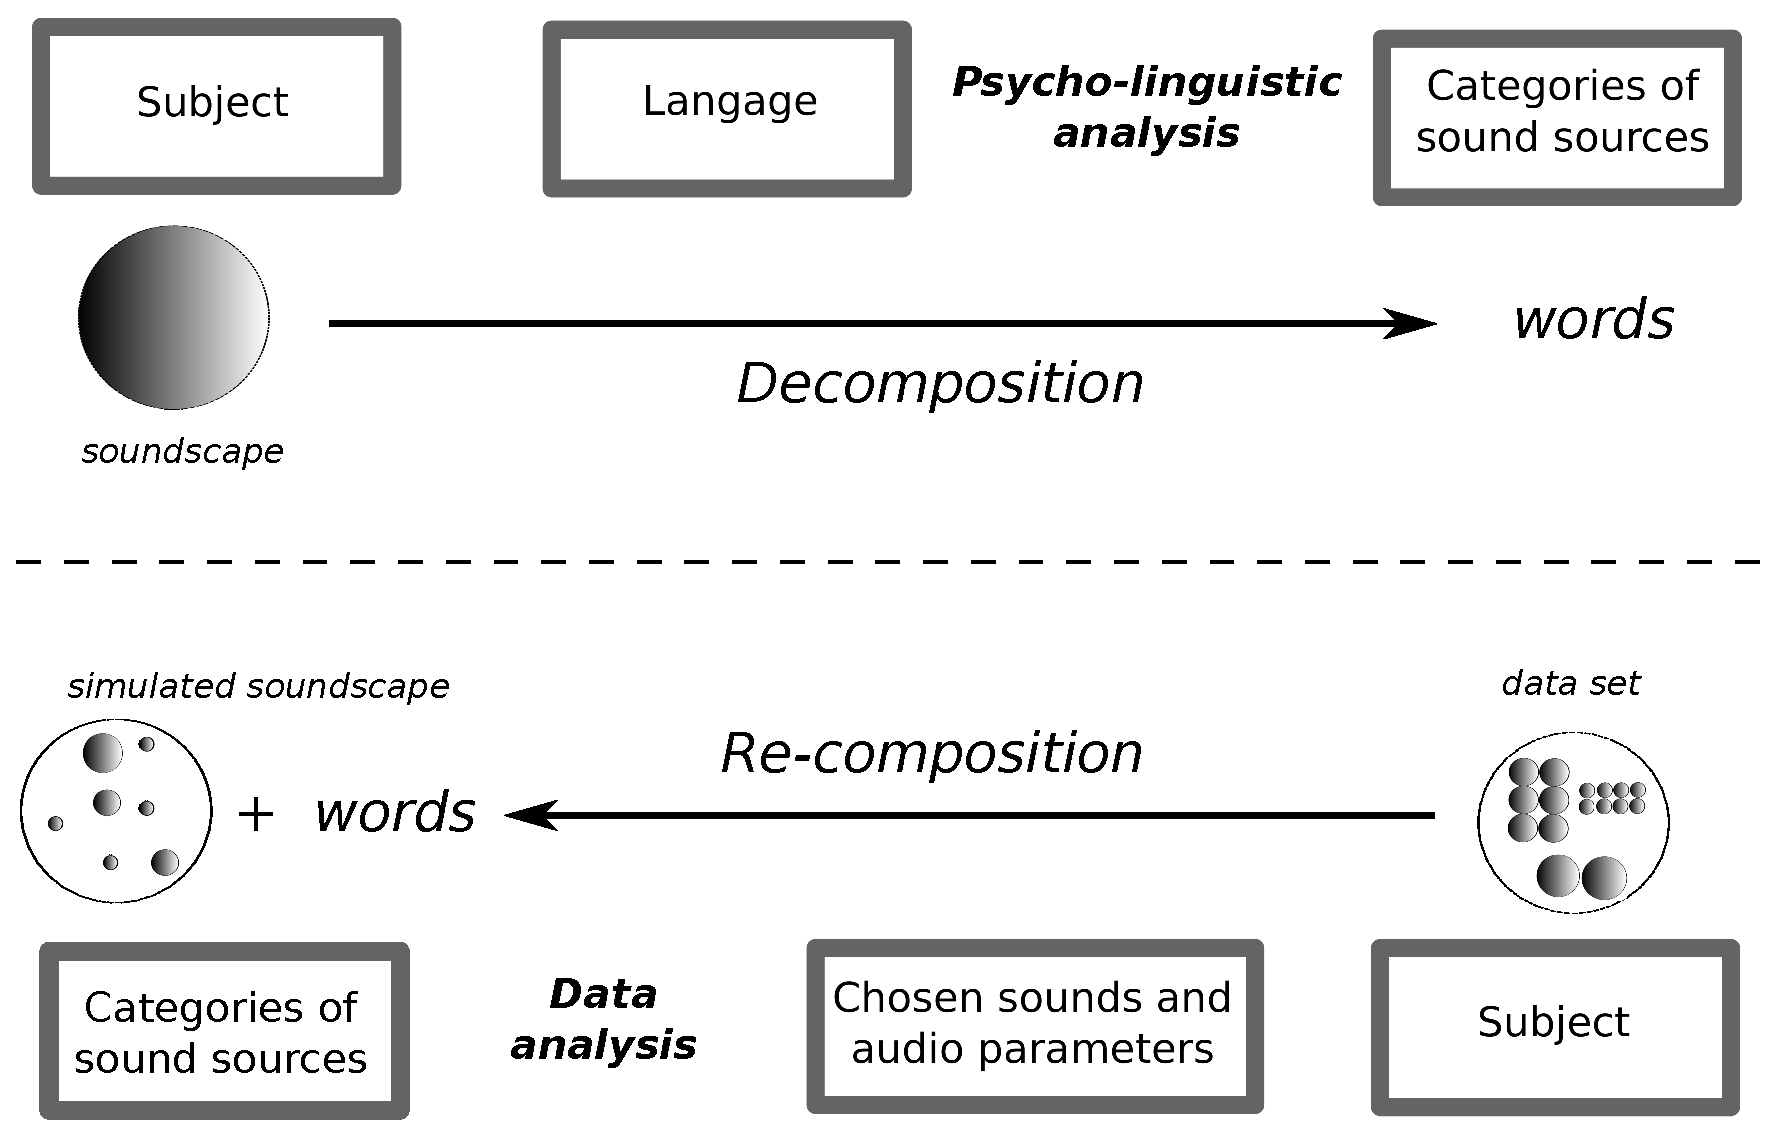
\includegraphics[width=.4\paperwidth]{../gfx/1.eps}
  \caption{\label{psycholing} Psycho-linguistic analysis paradigm (top) and proposed approach (bottom).}
  \end{center}
\end{figure}

\begin{figure}[t!]
\begin{center}
\includegraphics[width=.4\paperwidth]{../gfx/3.eps}
\caption{\label{datasetexample} Hierarchical structure of the event and texture data sets. Depending on the considered top class, there could be more or less than 3 semantic levels.}
\end{center}
\end{figure}

\subsection{Sample Selection process}

The sample selection process is designed to rely only on the listening of sounds themselves, in order not to influence subjects with \textit{a priori} associated semantic values. To explore the dataset without any written textual help, we have designed a selection interface where each leaf class is depicted by a point in 2D space. \gl{The interface performances are extensively tested in the following study} \cite{lafayJAES}. Subjects may only interact with the leaf classes of the datasets but the location of the points in space is constrained by the taxonomy, \textit{i.e.} subclasses belonging to a same class are close to one another. This organization is chosen to facilitate the sound class selection process and allow the subject to quickly apprehend the full range of the dataset. This may also reduce several potential biases of studies relying on verbal data to describe a soundscape: 1) the variable fluency of the subject in the experiment language, 2) the lack of definite terms to fully describe sounds or complex sound environments \cite{guastavino_ideal_2006}, and 3) the high inter-subject variability in the verbal description of a same sound.


\subsection{Simulation process and parameters}
\label{sec:simulationProcess}

Following the above described terminology, a soundscape is a sum of tracks. Each track is modeled by a temporal sequence of sound samples belonging to the same sound class. Thus, each track is related to one specific leaf sound class (see Section \ref{sec:SoundDataset}). To generate a soundscape, subjects may interact with the track parameters, but not with specific samples; for example, if a subject wishes to put a sequence of car sounds, he may specify how often (on average) cars pass by, and how loud they should be on average, but he cannot control each event individually. This allows to streamline the creation process, and keep the user focused on a global perception of the soundscape.

The simulation process involves two steps: 

\begin{enumerate}
\item \textit{Sound Class selection:}  the subject selects a leaf class of sound (``\,car passing\,'', ``\,heavy rain\,'', \ldots{}). Once a class is selected, a track made of randomly selected samples belonging to the considered sound class is created. For a texture track, samples are sequenced without any gap, using crossfades to guarantee seamless transitions. The soundscape simulator guarantees that a texture sample will never transition to itself in order to avoid any unnatural effect due to the repetition of identical sounds, that a human would easily detect \cite{agus_rapid_2010}.
\item \textit{Sound Class parametrization:} the subject may tune the parameters (time positioning and sound levels) of the track.
\end{enumerate}

Five audio parameters allow the subject to parametrize a track. The parameters always affect all the samples of a track and never a particular isolated sound. Two parameters, namely \textit{Inter onset spacing time} and \textit{Sample fade In/Out}, are only used with event tracks. 

\begin{enumerate}
\item \textit{Sound level} (dB): for each track, the sound levels of individual samples are drawn from a normal distribution. Subjects may control the sound level of a track by setting the mean and variance of the distribution. 
\item \textit{Global fade In/Out} (sec):  allows the subject to set a fade effect on the whole sequence of samples. 
\item \textit{Start and Stop position} (sec): allows the subject to set the beginning and the end times of a temporal sequence.
\item \textit{Inter onset spacing time} (sec): (event tracks only) similarly to the sound level, inter onset spacing times between events are drawn from a normal distribution that may be parametrized by the subject for each event track.
\item \textit{Sample fade In/Out} (sec): (event tracks only) allows the subject to set a same fade effect individually on each sample of an event track.
\end{enumerate}

Considering a soundscape as a sum of isolated samples is in line with the Auditory Scene Analysis (ASA) theory \cite{bregman1994auditory}, which states that auditory stimuli are decomposed into ``\,auditory objects\,'' called ``\,streams\,'', which may be regarded as sequences of auditory events emitted by putative sound sources \cite{ciocca2007auditory,winkler2009modeling}, and also with recent neuroscience studies suggesting that the primary auditory cortex (A1) produces representations of such ``\,auditory objects\,'' that act as bases for high level cognitive processing \cite{nelken2008neurons}. Thus, the track can be seen as the generative counterpart of the stream, which is rather a cognitive object.\nm{ce paragraphe est interessant mais est, a mon avis, mal place; il legitime la structure du simulateur, je le mettrais donc plutot dans le §3.1 en le developpant pt-etre un peu plus notamment les aspects neurosciences ...}

%%%%%%%%%%%%%%%%%%%%%%%%%%%%%%%%%%%%%%%%%%%%%%%%%%%%%%%%%%%%
%%%%%%%%%%%%%%%%%%%%   EXPERIMENT Plan %%%%%%%%%%%%%%%%%%%%%
%%%%%%%%%%%%%%%%%%%%%%%%%%%%%%%%%%%%%%%%%%%%%%%%%%%%%%%%%%%%

\section{Case Study: urban soundscape pleasantness}
\label{sec:CaseStudyUrbanSoundscape}
\subsection{Experimental planning}

We apply the proposed protocol to the field of urban soundscapes appraisal, by asking a panel of subjects to simulate two antagonistic urban soundscapes:  one ``\,ideal\,'', or pleasant (i) and the other ``\,non-ideal\,'' or unpleasant (ni) \nm{voir ma remarque en intro. sur la concordance ideal/pleasant ...}. The two labels have been chosen to compare the results with those of a previous study addressing ideal urban sound environment representations \cite{guastavino_ideal_2006}. The simulation protocol used in this experiment was previously tested and validated thanks to a pilot study~\cite{soundscape3}.

%run with 10 subjects.

To further characterize the simulated scenes, we run a complementary experiment where 10 subjects who did not take part in the first experiment are asked to evaluate the pleasantness of the simulated scenes using a bipolar semantic scale. This second experiment has two goals:

\begin{enumerate}
\item gain finer knowledge about the pleasantness of each simulated scene, \nm{trop vague a mon sens : a developper}
\item detect possible scene outliers. As the distinction i/ni \nm{cet encodage n'a  jamais ete defini avant - meme si on devine bien ce qu'il veut dire .... ;)} \gl{cf. plus haut} acts as our reference throughout the analysis, one has to ensure that all the scenes are indeed perceived as ideal or non ideal \nm{il ya confusion entre l'evalution ideal/non ideal et sur l'echelle de pleasantness .... est-ce la meme expe. ? a clarifier} scenes without ambiguity, \textit{i.e.} the highest average perceptual rating of the ni-scenes has to remain inferior to the lowest average rating of the i-scenes.
\end{enumerate}

The simulation experiment is referred as experiment-1 and the rating experiment as experiment-2. The complete experimental plan is described in Figure~\ref{fig:expLan}. \nm{Du coup, cette info; doit etre mise avant dans le paragraphe histoire d'evacuer toutes les confusions (cf. mes remarques plus haut)} \gl{non, je pense qu'à moins de deux paragraphes d'intervales, les lecteurs vont s'y retrouver.}

The simulated scenes as well as their annotations are available on an Archive Data Repository \footnote{\url{https://archive.org/details/soundSimulatedUrbanScene}}. Supplementary information including the experiment webpage and raw data for each experiment can be found on the companion website \footnote{\url{http://www.irccyn.ec-nantes.fr/~lagrange/demonstrations/simScene.html}}.

\begin{figure}[t]
\begin{center}
\includegraphics[width=.4\paperwidth]{../gfx/5.eps}
\caption{\label{fig:expLan} Experimental planning.}
\end{center}
\end{figure}

\subsection{Dataset of isolated samples}

The taxonomy, whose first two levels are depicted on Figure~\ref{fig:taxonomie}, is built following the category names found in previous studies addressing urban sound source categories \cite{maffiolo_caracterisation_1999,dubois2006cognitive,guastavino_categorization_2007, guastavino_ideal_2006, niessen_categories_2010, brown_towards_2011}, and is very similar to the one obtained in an other recent study on urban environmental sounds \cite{Salamon14}. 

483 monophonic urban environmental sounds are collected, including 381 sound events and 102 textures are chosen to build the dataset of isolated sound samples. Among them, 260 events and 72 textures are recorded by the authors using a \textit{Audio Technica AT8035} shotgun microphone (to isolate sounds from their background) connected to a \textit{ZOOM H4n} recorder. The remaining comes from existing sound banks \nm{preciser lesquelles ?} \gl{non}. All sounds are normalized to the same root mean square (RMS) level.

\begin{figure}[t]
\begin{center}
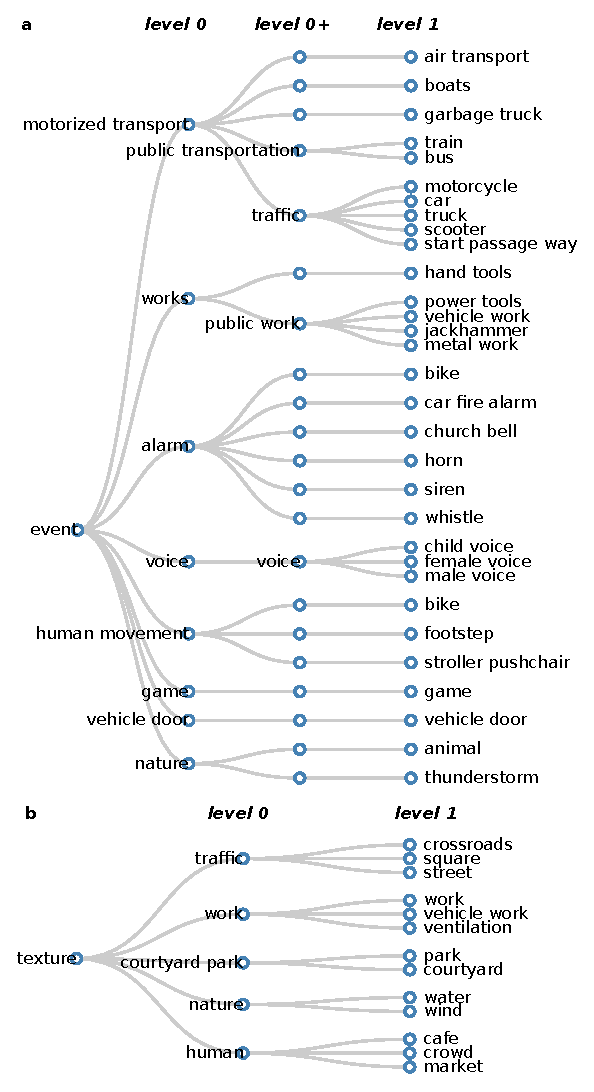
\includegraphics[width=.4\paperwidth]{../gfxHierarchy/taxonomy.eps}
\caption{\label{fig:taxonomie} Taxonomy of (a) sound events, and (b) sound textures for the semantic levels 0 and 1, as well as an intermediate grouping level denoted $0^{+}$.}
\end{center}
\end{figure}


%%%%%%%%%%%%%%%%%%%%%%%%%%%%%%%%%%%%%%%%%%%%%%%%%%%%%%%%%%%%
%%%%%%%%%%%%%%%%%  EXPERIMENT Set Up  %%%%%%%%%%%%%%%%%%%%%%
%%%%%%%%%%%%%%%%%%%%%%%%%%%%%%%%%%%%%%%%%%%%%%%%%%%%%%%%%%%%

\subsection{Set-up Experiment-1}
\subsubsection*{Procedure}

Subjects are asked to successively create two urban soundscapes, lasting one minute each. The first must be ideal (a soundscape in which the subject would like to live), the second non-ideal (one in which they would try to avoid living) \nm{reprendre la formulation exacte de la consigne} \gl{C'est la formulation, bien que cette dernière était transmise oralement}. They are asked to mimic a static listener. Subjects are not restricted in their design choices, but are forbidden to create physically impossible situations such as ``\,a dog barking every 10 milliseconds\,''. At the beginning of the experiment, a 20 minutes tutorial is planned in order to familiarize the subjects with the software environment. The experiment is scheduled to last from two to three hours.

Due to time constraints for the experiment-2, we trim 15 seconds from the start and end of each simulated scene, giving us 30 second scenes.

\subsubsection*{Participants and Apparatus}

44 post-graduate students (14 females) of the {\'E}cole Centrale de Nantes (French engineering school) take part in the experiment. They are about the same age (M: 21.6, SD: 2). All of them have been living in the same large French city (Nantes) for at least two years before the experiment. The experiment is run simultaneously with the 44 subjects spread into three identical rooms with a calm environment. Subjects are forbidden to talk to one another and asked to adjust volume to a comfortable level once, at the beginning of the experiment. Audio is presented diotically to each participant via headphones. Three experimenters are always present (one in each room) to give instructions and answer queries if needed.

Due to a misunderstanding of the instructions or a failure to proceed within the time limits, four subjects are excluded from the analysis. 40 subjects completed the experiment successfully, providing 40 ideal urban scenes (i-scenes) and 40 non-ideal urban scenes (ni-scenes). 

\subsection{Set-up experiment-2}
\label{sec:Experiment-2}
\subsubsection*{Procedure} 

Subjects are asked to evaluate the pleasantness of the 80 simulated scenes using a bipolar scale (also known as Likert scale) of 7 points going from -3 (non ideal, very unpleasant) \nm{a nouveau cet amalgame des 2 termes risque d'etre critiquee et doit etre argumenter et expliciter, je pense.} to +3 (ideal, very pleasant). The first ten scenes are used to give the subject an idea of the pleasantness range of the scenes. Those ten scenes are repeated at the end of the experiment and the ratings of their first occurrences are not taken into account in the analysis. Subjects listen to at least the 20 first seconds of the scenes and are free to skip the last 10 seconds at their convenience. Scenes are presented in a randomized order, but the ten calibration scenes are five i-scenes and five ni-scenes. \nm{also randomized in the presentation along subjects ?} \gl{a vérifier}

\subsubsection*{Participants and Apparatus}

10 post-graduate students (2 females) of the {\'E}cole Centrale de Nantes took part in the experiment. None of them did the first experiment. They are about the same age (M: 23.1, SD: 1.8). All of them have been living in the same large French city (Nantes) for at least two years. The experiment is run simultaneously with the 10 subjects in a calm environment. Audio is presented diotically to each participant via \textit{BeyerDynamic DT 990 Pro} semi open headphones at -12 dB (full scale). One experimenter is always present to give instructions and answer queries if needed. All the  subjects successfully completed the experiment. 

\subsection{Data analysis}

As experiment-1 generates a large amount of data suggesting numerous avenues of investigation, we here choose to restrict ourselves to the analysis of 1) selected sound classes, 2) sound event density, and 3) scene sound levels, other aspects being intentionally left for future research.

For ease of reading, we introduce the following terms and concepts that will be used throughout the analysis: 
\begin{description}
\item[$Diversity$:] number of distinct sound classes used in a scene. This number depends on the considered semantic level. For example, considering the two subclasses of the semantic level 2 \textit{car-passing} and \textit{car-starting}, which both belong to the same class \textit{car}, we count 2 distinct sound classes for semantic levels 2 and 3, but only 1 sound class for semantic levels 0 and 1. 
\item[$Density$ ($D$):] logarithm of the number of event samples per chunk of 1 second, averaged over the scene duration. Density may be computed considering all sound classes, or only a subset of them. If nothing is specified, then the density accounts for all classes. \gl{Empirically, we observed that the original distributions were skewed. The use of the logarithm compression allowed us to reduce this skewness.} 
\item[$Sound level$ ($L$):]  Decibel of the RMS voltage relative to 1 volt, computed every second and averaged over the scene duration. \nm{est-ce que cette reference correspond a une quelconque calibration du microphone
de prise de son (p. ex., X dB a 1 m.) ? Si oui, donner plus de details et expliquer comment tu as fait pour les samples issus de base de donnees - dont on ne connait pas a priori ces elements de calibration .....} \gl{non} An A-weighting filtering is performed before the RMS computation. Computing other statistical descriptors, namely the minimum, maximum or the 10-90th quantiles, shows that they all present a high correlation with the mean ($r\geq0.85$, $p<0.01$), therefore only the latter is considered.
\end{description}

We measure significance between the i- and ni-scenes using paired Student's t-test. All correlations are computed using the Pearson product-moment correlation coefficient. All statistical tests are performed at an $\alpha=5\%$ significance level.

%%%%%%%%%%%%%%%%%%%%%%%%%%%%%%%%%%%%%%%%%%%%%%%%%%%%%%%%%%%%
%%%%%%%%%%%%%%%%%  Results       %%%%%%%%%%%%%%%%%%%%%%%%%%%
%%%%%%%%%%%%%%%%%%%%%%%%%%%%%%%%%%%%%%%%%%%%%%%%%%%%%%%%%%%%
 
\section{Results}

\subsection{Validity of the  dataset and the selection interface}
\label{sec:datasetAnalyses}

The dataset and selection interface are now assessed by considering the subject comments. 

Looking at the database criticisms, 28 subjects stated that they could not find one or several desired sounds, with a maximum of 4 sounds for one subject. From all the missing sounds we identified 26 sound classes at different semantic levels. Among those classes, 16 were effectively present in the database, 1 referred to musical sounds which we had chosen to exclude from the database, and only 9 were effectively absent. Except for one sound class (``\,stroller pushchair\,''), each of the 16 classes which were reported as missing but were present in the database were used by at least one other subject. Among the 9 truly missing ones, we find very specific sounds as ``\,sport car\,'' or ``\,teenager voice\,''. We believe \nm{n'est-ce pas unpeu faible comme argumentaire ....? Pt-etre mettre les resultats en \% pour les rendre plus facilement intrerpretables ?} that those results show that the database diversity was sufficient for the purpose of the study. 

If we look at the interface criticisms, 32.5\% of all the subject clearly stated that the selection interface was a ``\,straightforward yet effective way\,'' to find a sound whereas only 10\% indicated that they encountered difficulties. The remaining 57.5\% did not report difficulties. 

Those results tend to confirm that both the data set and the selection interface are well suited for the experiment.

\subsection{Consistency of the data}

To ensure consistency of the simulated scenes, no ni-scene should be rated in average as more pleasant as any i-scene, and reciprocally. Figure~\ref{xp2_1}.a shows the distributions of the averaged ratings considering scenes as observations. Four scenes (2 i-scenes and 2 ni-scenes) appear to be ambiguous, and are henceforth removed from the analysis, as well as their antagonist scenes. This operation leaves us with 36 i-scenes and 36 ni-scenes. Corrected distributions are displayed on Figure~\ref{xp2_1}.b. Figure~\ref{xp2_1}.c shows the distributions of the averaged ratings, considering subjects as observations, without the scene outliers. It is clear that the pleasantness levels of the scenes, as intended by experiment-1 subjects, are well perceived by experiment-2 subjects ($p<0.01$).

\begin{figure}[t]
\begin{center}
\includegraphics[width=\columnwidth]{../gfxMatlab/xp2_1.eps}
\caption{\label{xp2_1} Boxplot of the averaged ratings given by the subject considering (a) scenes as observations, (b) scenes as observations without scene outliers and (c) subjects as observations without scene outliers. \nm{les figures sont petites et le chiox des couleurs contribue a leur faible lisibilite} \gl{?}} 
\end{center}
\end{figure}


\subsection{Density, sound level,  and diversity}
\label{sec:levelDensityDiversity}

\begin{figure}[t!]
\centering
\includegraphics[width=\columnwidth]{../gfxMatlab/xp1_deSoLv_1.eps} 
\caption{\label{fig:xp1_deSoLv_1}  Boxplot of (a) the scene densities ($D$) and (b) the scene sound levels ($L$). Scatter plot of (c) $D$ \emph{vs} ratings and (d) $L$ \emph{vs} rating}
\end{figure}


\begin{table}[t]
\centering
\begin{tabular}{l c c} 
                & $L$                          & $D$    \\
\hline
all             & \textbf{-0.76} ($p<0.01$)    & \textbf{-0.35} ($p<0.01$) \\
i-scenes        & -0.32 ($p=0.06$)             & -0.28 ($p=0.10$) \\
ni-scenes       & \textbf{-0.66} ($p<0.01$)    & \textbf{-0.47} ($p<0.01$) \\

\hline
\end{tabular}
\vspace{0.5mm}
\caption{\label{tab:numGlobal} Correlations computed between ratings \emph{vs} sound level ($L$) and event density ($D$)}
\end{table}

\begin{figure}[t!]
\centering
\includegraphics[width=\columnwidth]{../gfxMatlab/xp1_div_1.eps} 
\caption{\label{fig:analyseDensitySnrGlobal3} Diversity across semantic levels for event and texture classes. \nm{il faut mieux differencier les donnees provenant du corpus event et du corpus texture}}
\end{figure}

The event density ($D$) is slightly higher for ni-scenes than for i-scenes (Figure~\ref{fig:xp1_deSoLv_1}.a). The averaged $D$ are $1.2$ for the i-scenes, and $1.6$ for the ni-scenes, with a significant effect of the scene type ($p<0.05$). $D$ varies widely from subject to subject. 

Concerning the sound level (Figure~\ref{fig:xp1_deSoLv_1}.b), $L$ is significantly higher for ni-scenes than for i-scenes ($p<0.01$). 

To study the ability of those descriptors to characterize the appraisal, we compute the correlations between the ratings, $D$ and $L$, considering separately the i- and ni-scenes, as wel as all the scenes altogether. Results are shown in Table~\ref{tab:numGlobal} and in Figures~\ref{fig:xp1_deSoLv_1}.c and~\ref{fig:xp1_deSoLv_1}.d; \nm{pour rendre compte de cet effet, ne peut-on pas egalement calculer effectuer une MANOVA qui renseignera sur l'interaction de 1er ordre entre la variable dependante (ratings) et les variables independantes / facteurs expe. (density et Leq) ?} \gl{NM comments: je ne pense pas qu'une MANOVA s'utilise comme cela, comme toute analyse de variance, la variable independante est categorielle. De plus dans une MANOVA, le M de multivarié s'applique aux variales dépendantes, la proposition relève de la two way anova (mais le rating étant continu cela ne marche pas). Il faudrait faire une regression multiple avec terme d'interaction P=A+B+A*B, et interpréter A*B...}

Not surprisingly, these results show that ni-scenes are on average louder than i-scenes. The strong correlation of $-76\%$ between $L$ and the ratings indicates that the sound level does influence the pleasantness. However, the correlations computed separately for the i- and ni-scenes suggest $L$ does not characterize the notion of pleasantness in a equal manner for the two type of scenes:  there is still a good correlation between $L$ and the ratings for the ni-scenes, but there is no correlation if we take only the i-scenes. This is in line with the trend observed by \cite{lavandier2006contribution} that sound level may be a sufficient indicator of comfort for negatively rated acoustics scenes, but not for positively rated ones.

\gl{Considering the event density, ni-scenes seem to be slightly more populated that i-scenes. However, the weak correlation between $D$ and the ratings ($-0.35$) shows that a global measure of $D$ fails to characterize the appraisal if all the scenes are considered altogether. If we consider the two types of scenes separately, the correlation remains moderate for the ni-scenes, and is non-existent for the i-scenes. This may suggest that either the number of events is an irrelevant indicator, or that only the densities of specific event classes are involved. Still, although there is no clear correlation between $D$ and pleasantness for the ni-scenes, $D$ seems to play an indirect role as it is correlated with $L$ ($0.62$, $p<0.01$). In other words, $D$ does have an impact on the appraisal only when the addition of new events increases the sound level.}

Averaged diversities are shown on Figure~\ref{fig:analyseDensitySnrGlobal3}. Except for semantic level 0, the diversity is significantly higher for the event classes of the ni-scenes (levels 1, 2 and 3: $p<0.01$;), revealing that ni-scenes are composed of a larger variety of sound events than i-scenes. Diversity remains constant across semantic levels for texture classes of i- and ni-scenes, with no statistical differences. \nm{qu'en est-il pour les classes event ? Est-ce que les differences observees sur fig. 7 (a partir de semantic level 1) sont statist. siginificatives ?} \gl{cf. phrase précédente} The correlations computed between the event diversities and the averaged pleasantness ratings remain weak or moderate ($r<0.45$ \nm{r = 0.45 ?} \gl{NM comments: non, toutes les correlations sont inf à .45}, $p<0.01$), irrespective of the considered semantic level.  If we look at the two types of scene separately, no correlation is observed. \gl{Although the diversity varies between the i- and ni-scenes, this last result shows that it is not a good indicator to precisely characterize the pleasantness.}


\subsection{Class selection}
\label{sec:classSelection}

We investigate the sound class selection by counting the number of times a class has been used to simulate the i- or ni-scenes. Figures~\ref{fig:xp1_class_1}.a and~\ref{fig:xp1_class_1}.b  shows the class distributions for the event and texture classes, respectively. For ease of reading, we choose an intermediate semantic level, denoted $0^{+}$, laying between semantic levels 0 and 1 (see Figure~\ref{fig:taxonomie}).

There is a considerable difference between the sound class selections of the i- and ni-scenes, showing that semantics play an important role in soundscape qualitative evaluation. The sound classes shown in Figures~\ref{fig:xp1_class_1}.a and~\ref{fig:xp1_class_1}.b are very close to those found by Guastavino \cite{guastavino_ideal_2006}, \textit{i.e.} classes that suggest human presence and nature are the most present in i-scenes while classes referring to mechanical and construction work sounds are used for ni-scenes.

\gl{However, some differences have to be reported: \cite{guastavino_ideal_2006} reports that ``\,public transports\,'' are typical sounds of an ideal urban environment. This observation is attributed to the fact that urban environment perception is driven by social considerations. Public transport sounds are thus better accepted than those of private vehicles, as they are usually positively connotated. Results shown in Figure~\ref{fig:xp1_class_1}.c tend to qualify this claim  by showing that sounds of public transports (\textit{bus} and \textit{train}) were chosen by $28\%$ of the subjects for the i-scenes and by $42\%$ of the subjects for the ni-scenes. It is important to note that in \cite{guastavino_ideal_2006} subjects are asked to recall an environment in memory, that is, without any sound support. Tacking the reality of the sound into account, results show that public transport sounds cannot be considered as peculiar to an ideal urban soundscape. The class \textit{public\_transport} does appear in ni-scenes, more than \textit{car} or \textit{truck}. Similar findings showing that bus presence may have a negative effect on soundscape appraisal are reported in \cite{lavandier2006contribution}. One should note that the data still does not contradict the idea that public transport sounds are well accepted: \textit{bus} sounds were chosen by $25\%$ of the subjects for the i-scenes, circa as much as \textit{bike} sounds and more than any other vehicle sounds. }

\begin{figure*}[t!]
\begin{center}
\includegraphics[width=2\columnwidth]{../gfxMatlab/xp1_class_1.eps}
    \caption{\label{fig:xp1_class_1} (a) Percentage of subjects using (a) event sound classes of the semantic level $0^{+}$, (b) texture sound classes of the semantic level $0^{+}$ and (c) event classes of the semantic level 1 belonging to the event classes \emph{traffic} and \emph{public transport} of the semantic level $0^{+}$; ni-scenes (left-red), i-scenes (right-green).}
\end{center}
\end{figure*}

%\begin{figure}[t!]
%\begin{center}
%\includegraphics[width=.4\paperwidth]{../gfxMatlab/xp1_class_2.eps}
%    \caption{\label{fig:xp1_class_2} Percentage of subjects using  to simulate the i-scenes (left-green) and the ni-scenes (right-red).}
%    \end{center}
%\end{figure}

\subsection{Markers}
\label{sec:markers}

As semantics is found to play an important role in the qualitative perception of the soundscape, we now investigate the existence of sound markers \nm{est-ce l'accepation de Schafer ? d'apres ce qui est ecrit juste apres je ne pense pas; par contre, d'apres ce qui est ecrit un peu plus bas (en citant justement Schafer) ca peut l'etre .... Il y a ici une ambiguite sur le terme qu'il serait bon de clarifier.} \gl{Non ce n'est pas  l'interprétation de Schaffer, on expliquait plus en détail avant les termes, mais c'est trop long, et non necessaire pour la compréhension du papier}, \textit{i.e.} sound classes of great importance when considering the pleasantness of a soundscape. Here, an event class is considered as a marker if it has been mostly used in one type of soundscape (i or ni). To identify markers, a two-tailed V-test statistical test is performed for each semantic level. The V-test tests the null hypothesis that the $n_k$ event classes used for the scene type $k$ are randomly drawn from all the $n$ event classes available. A rejection of that hypothesis provides evidences that an event class has been significantly used for one type of scene only. Since the test concerns many event classes, Bonferroni correction is applied.

Results are shown on Table~\ref{tab:markers}. Nine markers are found across all semantic levels. As suggested by Figures~\ref{fig:xp1_class_1}.a, sounds evoking human activity (\textit{male footsteps concrete}) and nature (\textit{animal}, \textit{birds} and \textit{birds singing}) are markers of the i-scene. The presence of \textit{church bell} and \textit{bell bike} as strong markers of the i-scenes can be due to the socio-cultural background of the subjects, in great majority European citizens. It confirms Schafer's claim that sounds that are recognized by a community as integral part of its sonic environment are popular \cite{schafer1977tuning}. 

Markers of the ni-scenes are sounds due to construction work (\textit{construction work}), and sounds suggesting dense traffic (\textit{horn}, \textit{siren}). Although these markers are rather intuitive, none of the event classes related to motorized vehicles is a marker. It seems that subjects chose to illustrate unpleasant traffic sounds using horns and sirens.

\begin{table}[t]
 \setlength{\tabcolsep}{0.2pt}
 \centering
  {\renewcommand{\arraystretch}{0.9}
\begin{tabular}{c c c c} 
Semantic   &  \multicolumn{2}{c}{Markers} \\
level & i-scenes & ni-scenes \\
\hline
0  &                               &  construction work (3.78)  \\
\hline
  & church bell  (4.5)             & horn  (3.9) \\
1 & bell bike    (4.3)             & siren (3.9)\\
  & animal       (4.2)             &       \\
   \hline
  & birds        (4.8)             & horn  (4.0)\\
2 & church bell  (4.4)             & siren (4.0)\\
  & bell bike    (4.2)             &       \\
   \hline
  & birds singing (4.8)            & horn  (4.1)\\
  & church bell   (4.3)            & siren (4.0)\\
3 & bell bike     (4.2)            &       \\
  & male footsteps                 &  \\
  &   concrete (3.6)               &  \\
  \hline
\end{tabular}
}
\vspace{0.5mm}
\caption{\label{tab:markers} Event classes found to be markers. In each cell, markers are ordered from top to bottom by decreasing V-test values.}
\end{table}

\subsection{Quantifying class selection}
\label{sec:QuantifyingClassSelection}

\begin{figure}[t]
\begin{center}
\includegraphics[width=\columnwidth]{../gfxMatlab/pa5_1.eps}
\caption{\label{fig:pa5} Precision at rank 5 ($P@5$) computed from the \textit{Hamming} distances between the scenes at different semantic levels, considering the event and texture classes ($ET$), the event classes ($E$), the texture classes ($T$), the event markers ($E_m$) and event classes without event markers ($E_{w/o,m}$) .}
\end{center}
\end{figure}

To quantify how class selection characterizes the pleasantness of a urban environment, we now follow a class-based classification of the scenes evaluated with the standard precision at rank 5 ($P@5$) metric. 

Each simulated scene $s_i$ is represented by a boolean vector of dimension $n$: $S_i = (x_1, x_2, \ldots{}, x_{n})$, $i=\lbrace 1, \ldots, 72 \rbrace$. Each dimension corresponds to a sound class (event and texture) of a particular semantic level (for example: $n=44$ classes for semantic level 1). Thus $x_1 = 1$ indicates that the sound class $x_1$ is present in scene $s_i$ (not present if $x_1=0$). A \textit{Hamming} distance is computed between all pairs of $S_i$. Then, for each scene $s_i$, the number of scenes sharing the same label (i or ni) among the five scenes $s_j$ that have the smallest distance to $s_i$ is computed. The $P@5$ precision is then obtained by averaging the results over the 72 scenes $s_i$.

Results considering both the event and texture classes ($ET$) \nm{symbolisme pas clair} \gl{pk ?} to build the vectors  $S_i$ are shown on Figure~\ref{fig:pa5}. The $P@5$ is of 76\% for semantic level 0 and remains above 86\% starting at semantic level 1. These result strongly indicates that it is possible to make a clear distinction between the i- and ni-scenes based solely on the class presence/absence. We also note that the deeper the hierarchical level, the higher the $P@5$; in other words an increased precision in identifying scene elements allows a better distinction between i- and ni-scenes. 

To refine the analysis, only event classes ($E$), texture classes ($T$), event markers ($E_m$) and event classes without event markers ($E_{w/o,m}$) are also considered on Figure~\ref{fig:pa5}. The constant deviation of circa $15\%$ from the semantic level 1 between $E$ and $T$, and the fact that $P@5$ are similar for $ET$ and $E$ indicate that soundscape quality is mostly conveyed by sound events.

Since similar precision are achieved by $ET$, $E$ and $E_m$, we may conclude that all the event classes are not equivalently important to distinguish between the two scene types. Indeed, $E_m$ uses very partial information but still reaches quasi-equivalent results. Moreover, the drop in $P@5$ considering $E_{w/o,m}$ from the semantic level 1 confirms the fact that soundscape quality mostly relies on the presence of specific sound markers.


\subsection{Marker-wise pleasantness descriptors}
\label{sec:QuantifyingMarkers}

\begin{table}[t]
\centering
\begin{tabular}{l r r} 
                    &   i-scenes   & ni-scenes \\
\hline
$L_m$         & 0.19  ($p=0.28$)           & \textbf{-0.60} ($p<0.01$) \\
$L_b$         & \textbf{-0.51} ($p<0.01$)  & -0.16 ($p=0.36$) \\
$L_{m-b}$     & \textbf{0.69} ($p<0.01$)   & -0.31 ($p=0.06$) \\
$D_{m}$       & -0.20  ($p=0.24$)          & \textbf{-0.58} ($p<0.01$)  \\
$D_{b}$       & -0.23  ($p=0.18$)          & -0.30 ($p=0.07$)  \\
\hline
\end{tabular}
\vspace{0.5mm}
\caption{\label{tab:numMarkers} Correlations computed between rating \emph{vs.} $L_m$, $L_b$, $L_{m-b}$ and $D_m$.}
\end{table}

\begin{figure}[t]
\begin{center}
\includegraphics[width=.4\paperwidth]{../gfxMatlab/xp1_deSoLvMar_1.eps}
  \caption{\label{fig:numMarkers} Averaged pleasantness vs. (a)  $L_{m-b}$, (b) $L_{m}$, (c) $L_{b}$ and (d) $D_m$.}
  \end{center}
\end{figure}

In order to check if the physical characteristics of the markers alone have an influence on the pleasantness, we now compute $D$ and $L$ considering on one hand the tracks of the markers ($L_m$, $D_{m}$) only, and on the other hand the remaining of the sounds ($L_b$, $D_b$). As the marker durations are rather short, and the number of markers in a scene rather low, a window length of 125 ms is used to compute $L_m$ and $L_b$ \nm{pourquoi cette precision methodologique n'a t'elle pas ete donnee aussi au moment de definir ce parametre ?} \gl{non, elle change ici}. The difference $L_{m-b}=L_m-L_b$ is also considered as it illustrates how the markers emerge from the other sounds. Correlations between those descriptors and the average ratings are depicted in Table~\ref{tab:numMarkers} and Figure~\ref{fig:numMarkers}.

Considering $D_{m}$ (Figure~\ref{fig:numMarkers}.d), results are almost the same than to those found in section~\ref{sec:levelDensityDiversity}. There is no correlation for the i-scenes, but the correlation increases for the ni-scenes. No correlation is found for $D_{b}$. Sound levels descriptors are much more informative. Little to no information is lost by considering only the markers to compute $L_m$, \emph{i.e.} there is still a good correlation for the ni-scenes (although inferior to the one observed in Section~\ref{sec:levelDensityDiversity}), and no correlation for the i-scenes.

Considering the ni-scenes, the good correlation for $L_m$  (Figure~\ref{fig:numMarkers}.b) and the absence of correlation for $L_{b}$  (Figure~\ref{fig:numMarkers}.c) suggest that sound levels of the ni-markers convey most of the unpleasantness. The fact that no correlation is observed for $L_{m-b}$ (Figure~\ref{fig:numMarkers}.a) indicates that the predominant influence of the marker sound levels remains true irrespective of the sound level of the other sounds. A loud horn sound is expected to increase the annoyance level of a scene (more so than a soft klaxon sound), whether or not the remaining of the sonic environment is ``\,noisy\,''.

That said, this last statement is not valid for the i-scenes. The strong uphill correlation found between pleasantness and  $L_{m-b}$ (Figure~\ref{fig:numMarkers}.a) shows that the higher the markers sound levels relative to the other sounds, the higher the pleasantness. But the moderate downhill correlation observed for $L_{b}$ (Figure~\ref{fig:numMarkers}.c) shows that the levels of those remaining sounds may be a cause of annoyance if perceived as too loud. It is thus the emergence of the i-markers from the others sounds that drive the appraisal. Considering for example the sonic environment of a park and following those conclusions, the global appraisal will increase with the sound level of the birds, provided other sounds like human voices or traffic hubbub are not too loud.

These results are strong indicators that global sound level alone is not sufficient to properly characterize the appraisal of \emph{a priori} positive sound environments such as a park or a quiet street. On the contrary, the contribution of each sound source needs to be considered separately, as for certain type of sounds, the pleasantness does increase with their sound levels.

Those observations may also serve as guidelines for urban planner, showing that:

\begin{itemize}
\item in the case of negative environment such as street with public work or busy traffic, where it is often difficult to diminish the global sound level, focusing only on the noise regulation of specific sound sources (jack-hammer or horn) may significantly reduce the overall annoyance;
\item in the case of positive environment such as park or quiet street, the appraisal may be enhanced by increasing the presence of specific sound sources such as birds singing.
\end{itemize}

\nm{n'est ce pas au bout du compte, 2 propositions contraposees qui reviennent a dire qu'il faut au 1er ordre s'interesser a certaines sources particulieres (et a leur niveau) plutot que considerer un percept global (notamment en terme de niveau)} \gl{rien compris}
%%%%%%%%%%%%%%%%%%%%%%%%%%%%%%%%%%%%%%%%%%%%%%%%%%%%%%%%%%%%
%%%%%%%%    DISCUSSION AND PERSPECTIVES   %%%%%%%%%%%%%%%%%%
%%%%%%%%%%%%%%%%%%%%%%%%%%%%%%%%%%%%%%%%%%%%%%%%%%%%%%%%%%%%

\section{Discussion and perspectives}


We introduce in this paper a novel experimental protocol to study the perception of soundscapes, where subjects are asked to recreate an auditory environment using a tool specifically developed for that purpose and a structured database of isolated sounds. This protocol allows us to generate soundscapes whose composition, in terms of nature, timing and intensity of sound sources, is known with perfect accuracy. Using the data thus produced in a series of analyses on the issue of ideal \emph{vs} non-ideal urban soundscape classification and characterization, we showed that:

\begin{itemize}
\item The data obtained with the simulation allows us to reach results that are consistent with previous perceptual studies relying on recorded scenes \cite{lavandier2006contribution} or the experimental subjects' memory \cite{guastavino_ideal_2006}.
\item From the global descriptors sound level, class diversity and event density, only sound level seems to play a role in pleasantness evaluation.
\item The ability of sound level to characterize pleasantness relies upon the quality of the scene itself. For positively rated scenes (i-scenes), it is not relevant.
\item A semantic description of the soundscapes in terms of presence~/ absence of sound sources is an effective criterion to distinguish between ideal and non-ideal urban environments.
\item A few event markers, appearing at various semantic levels, suffice to perform efficient discrimination between ideal and non-ideal urban environments, although the type of markers found in this study may depend on the socio-cultural background of the subjects. 
\item The sound level computed on the markers only is a better predictor of perceived agreement than the global sound level.
\end{itemize}

Compared to more traditional survey based methods, the proposed method provides an increased precision and reliability of soundscape description useful for the analysis of subjects' judgments. This article was intentionally focused on the analysis of the scene composition; further research shall be dedicated to 1) a thorough study of the influence of the physical characteristics of the sound markers on pleasantness evaluation, as well as categorisation process, and 2) the elaboration of a predictive method based on that analysis, allowing to anticipate the agreement \nm{encore un autre terme : synonyme de pleasantness ?} of an acoustic environment from its composition.

In addition, more understanding shall be gained about the actual impact of sound level on soundscape perception: is there a significant difference in evaluation between two scenes having the exact same composition, but different levels? Is loudness but a consequence of scene composition ? \nm{cette derniere phrase est incomprehensible .... bien qu'elle semble importante car elle introduit la notion de loudness (perceived intensity) en oppposition a la notion de sound level (measured intensity) utilisee jusqu'a present : a eclaircir et approfondir davantage, je pense .....}

\nm{je ne suis pas trop du genre a raisonner comme cela mais je me dis que : vu le type de revue (AAA) et la thematique de l'article , il est possible que nous ayons JD. Polack comme potentiel reviewer, or nous ne citons aucun de ses travaux en la matiere ......}

\noindent \textbf{Acknowledgements}\\
\setlength{\parindent}{0.7cm} 
Research project partly funded by ANR-11-JS03-005-01. The authors would like to thank the students of the Ecole Centrale de Nantes for their willing participation.

%----------------------------------------------------------------------------------------
%	REFERENCE LIST
%----------------------------------------------------------------------------------------


\References{}{../biblio}{actalit}



\end{document}
